\noindent Social interaction---meeting a friend for a coffee or meal, chatting with co-workers in the workplace, or even small-talk with neighbors and shopkeepers---is ingrained in the daily life of many city dwellers. However, when the COVID-19 pandemic began in 2020, face-to-face social interactions largely disappeared as public health authorities discouraged meeting with people from other households. Later, once outdoor transmission of the virus was deemed unlikely while following social distancing guidelines, public spaces could again be used for social interaction. This research proposes how city parks could have been maximized---and how they can be maximized in the future---as a low-risk space for city residents to maintain social activity during a public health crisis. The existing capacity of outdoor social gatherings will be quantified and compared to the population of the surrounding areas for three notable city parks: Hyde Park in London, England; Prospect Park in New York City, United States; and Yoyogi Park in Tokyo, Japan. 

\begin{multicols}{2}

\section{Motivation}
Motivation for this research comes from personal experience and observations during the first few months of the COVID-19 pandemic. I lived in an apartment in San Francisco with no outdoor space and windows that hinged open a couple of inches. Golden Gate Park, the 1017-acre (4.12 square kilometers) expanse of greenery in the middle of the city, was half a mile (800 meters) away, but for the first month of the pandemic I left home only once per week to go grocery shopping then quickly return home. By the second month I was taking daily walks in the park or in the neighborhood, wearing a mask even when there were no other people in sight. In the summer of 2020 I would meet friends in Golden Gate Park and, sitting more than six feet apart, we would enjoy the fresh air and each other's company for hours despite the chilly San Francisco weather. 

In urban environments where residents do not have private outdoor space, city parks are a place to experience nature, exercise, and socialize \cite{geng_impacts_2021}. These are common activities even without a pandemic. That said, during so-called "normal times" city residents and tourists have many other entertainment options, making parks less likely to reach capacity. During a pandemic, in-person social activities suddenly become carefully planned, contact-traceable events with decreased frequency but perhaps increased duration \cite{sundara_rajoo_addressing_2021}. Two methods to mitigate infection risk from social interactions are avoiding social contact altogether and meeting in conditions where disease transmission is less likely which, in the case of COVID-19, is outside.  

Living within a ten-minute walk of Golden Gate Park, I came to rely on picnics with friends to fulfill my social needs during the pandemic. Groups as small as two to ten or more friends would gather, regardless of the weather, each household setting up their own blanket and bringing their own food (see Figure \ref{fig:golden_gate}). Such practices inspired this research project. The foregoing data and analysis show that quantifying even something as inexplicable as a picnic in a park could potentially help our cities prepare for the next public health crisis.   

\end{multicols}

 \begin{figure}[h!]
  \centering
  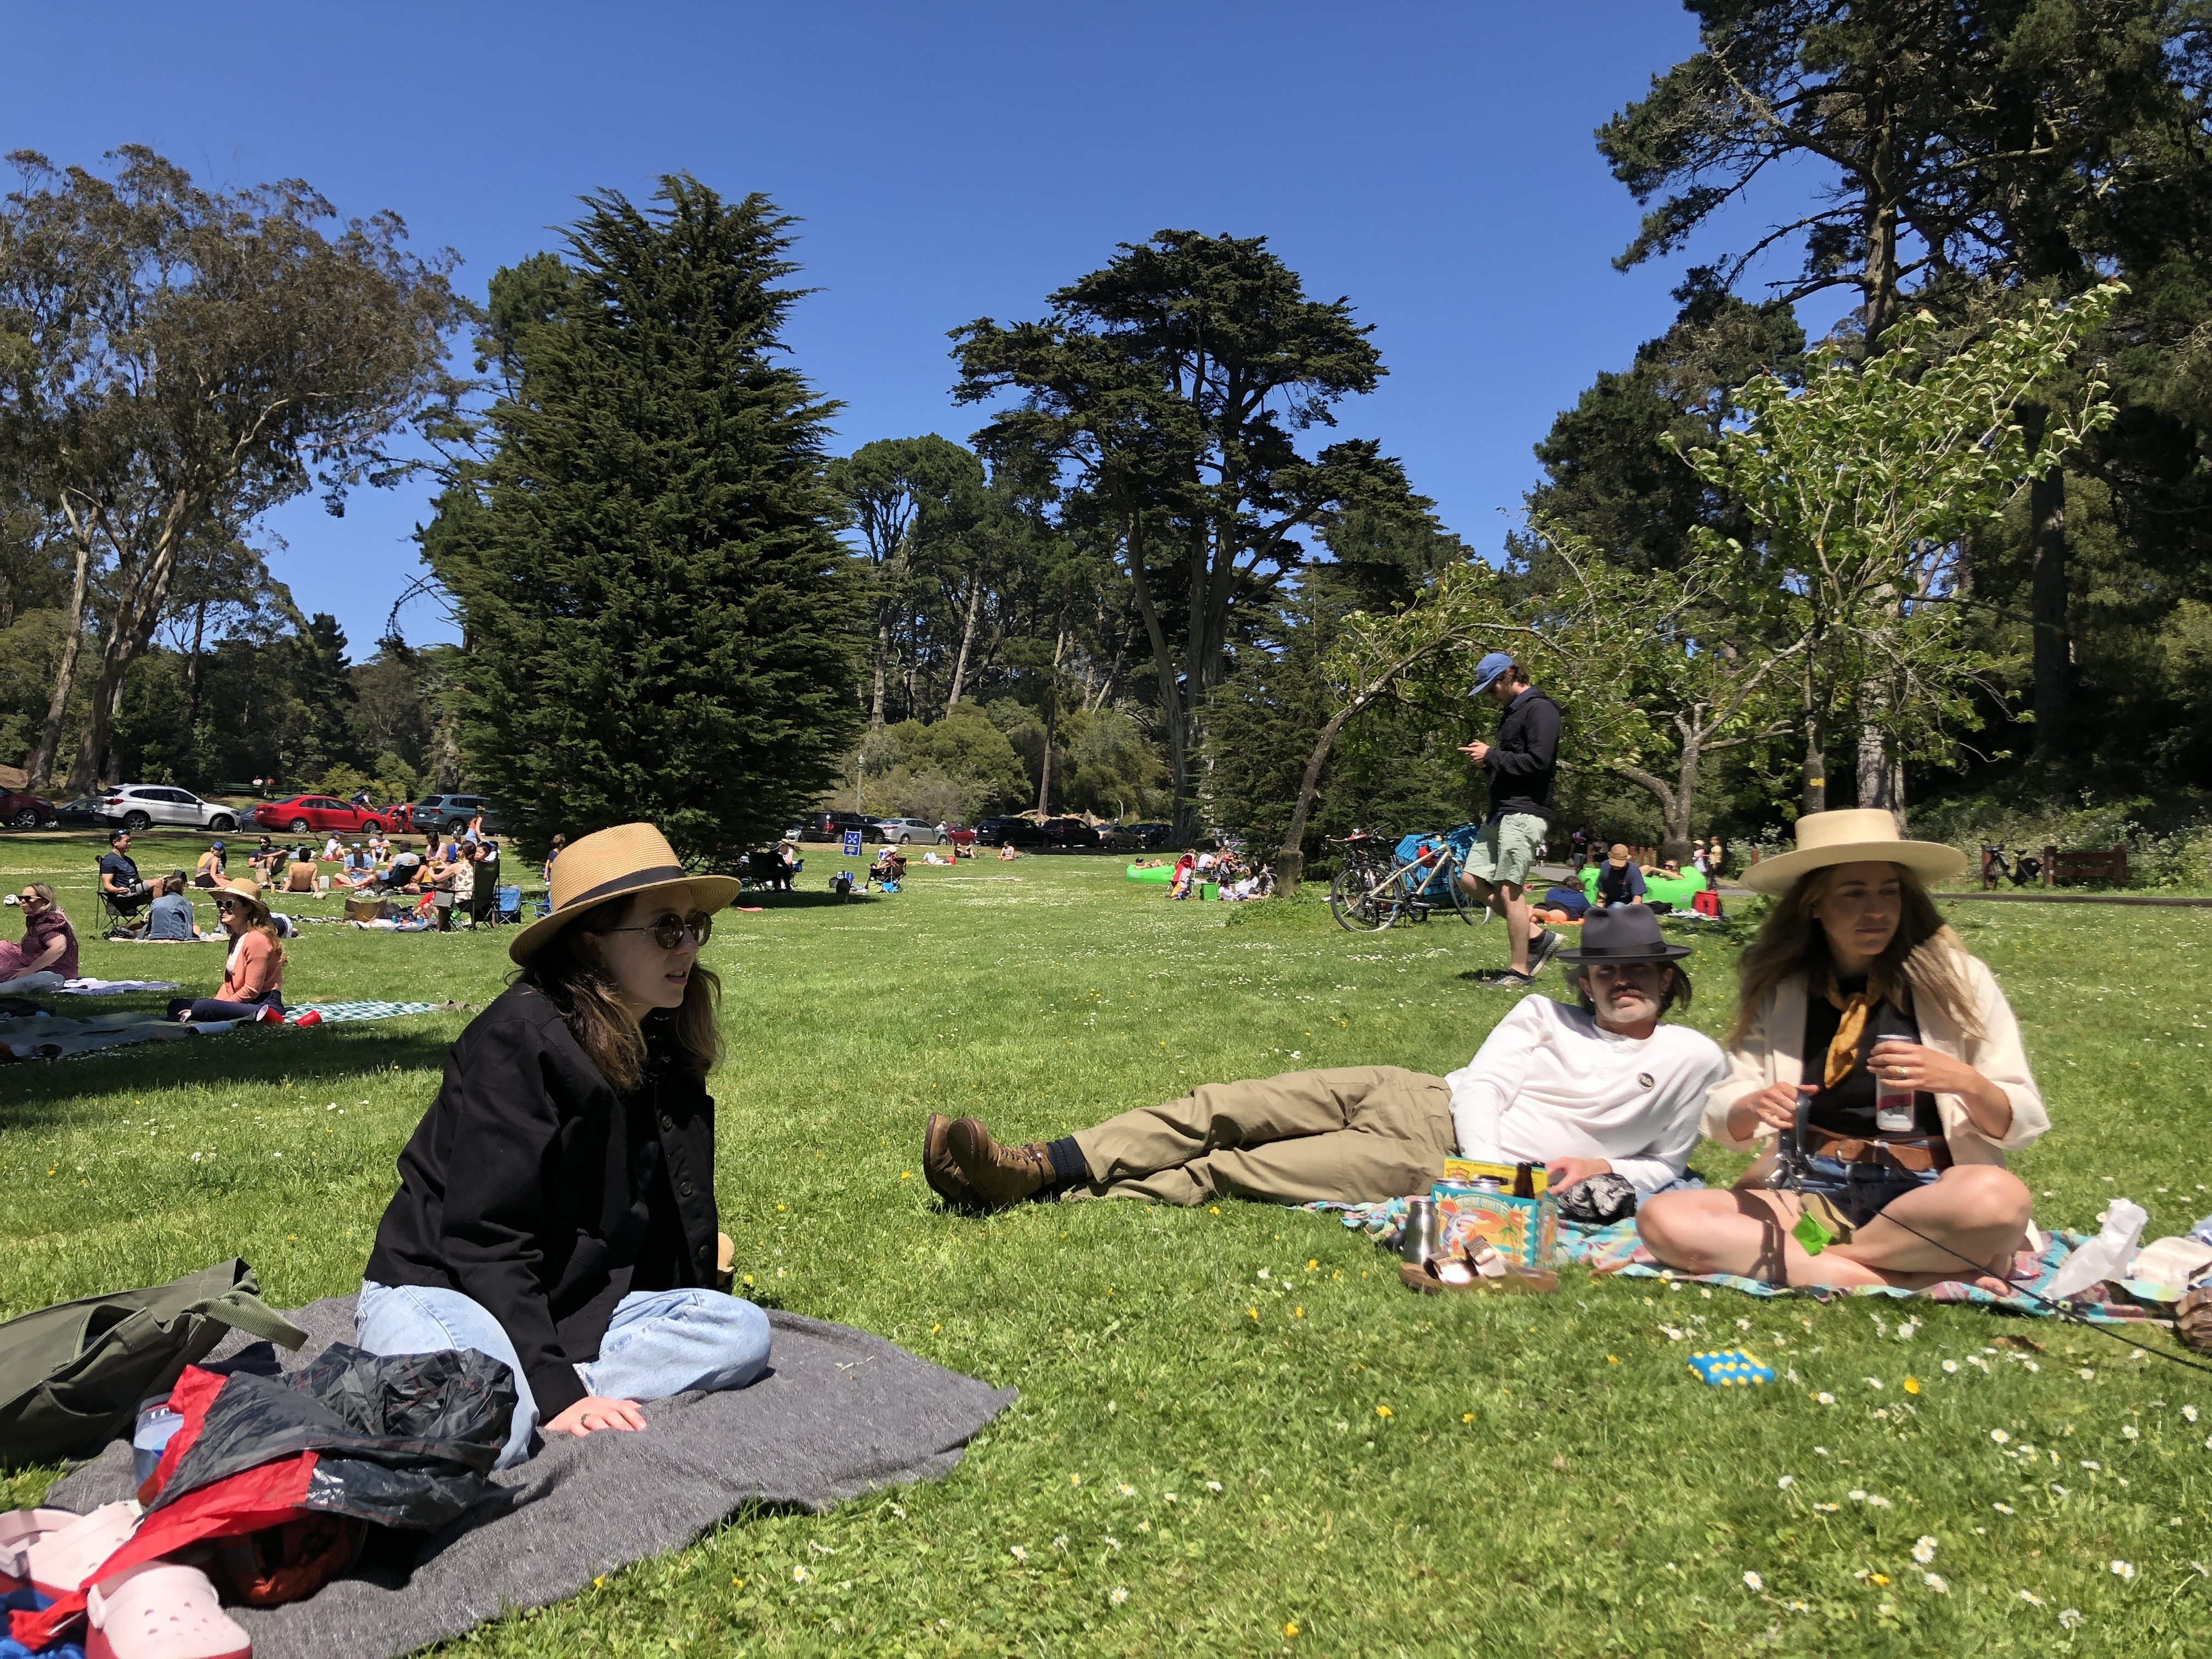
\includegraphics[width=0.8\textwidth]{images/introduction/ggp.jpg}
  \captionsetup{width=0.8\linewidth}
  \caption[Golden Gate Park]{Outdoor social gatherings in Golden Gate Park in San Francisco, United States, taken in May 2020 by the author.}
  \label{fig:golden_gate}
\end{figure}

\begin{multicols}{2}

\section{Background}
\subsection{"The pandemic"}
As known cases of SARS-CoV-2, colloquially referred to as COVID-19 or Coronavirus, started to increase in the spring of 2020, urban areas around the world came to a standstill. Normally traffic-clogged roads were empty, shops and restaurants closed, and the few people out walking dogs or picking up groceries protected themselves from infection by wearing masks, goggles, and gloves. From March through June 2020 in New York City, the urban chaos caused by COVID-19 was concentrated inside hospitals pushed to their limits to save patients from the new virus that proved to be fatal for 9.2\% of infected people and 32.1\% of hospitalized patients \cite{thompson_covid-19_2020}.

According to Merriam Webster, the words added to their lexicon in March and April 2020 included: COVID-19, community spread, social distancing, physical distancing, super-spreader, contactless, and more \cite{noauthor_coronavirus_nodate}. Social distancing, for example, is defined by Merriam Webster as "the practice of maintaining a greater than usual physical distance (such as six feet or more) from other people or of avoiding direct contact with people or objects in public places during the outbreak of a contagious disease in order to minimize exposure and reduce the transmission of infection" \cite{noauthor_social_nodate}. The addition of these words shows just how quickly the world of face-to-face interactions became a threat to human existence.  

Furthermore, public health directives not only discouraged in-person social interactions but in some cases enforced it with lockdown measures, travel restrictions, and curfews \cite{geng_impacts_2021}. The use of public spaces was prohibited, events were canceled, public transportation was to be taken sparingly, and school and work places transitioned to be fully remote. Citing the mental health consequences of limiting social interaction, the term “social distancing” was called into question by Thomas Abel and David McQueen in their March 2020 editorial for the International Journal of Public Health \cite{abel_covid-19_2020}. The authors called for a change in semantics, from social distance to spatial distance. Spatial distance refers to the public health advice of maintaining a two meter distance between people from different households, but the authors encouraged creative ways of nurturing social closeness to prevent the above-mentioned consequences of severing all social ties in the face of a long-term public health crisis.

For those without personal vehicles, the sudden shift to remote working and reduced public transportation service left only the amenities accessible by foot. Moreover, due to the unknown nature of the infectious disease, many people avoided leaving their homes altogether and there was an immediate increase in grocery delivery and restaurant takeout orders as a result \cite{wang_adoption_2021}. As more epidemiological information was known about COVID-19, people began seeking ways to see friends and family while maintaining the advised six-foot (two-meters) “social distance.” Those with backyards could host friends and family outdoors while maintaining the recommended distance, but this was generally limited to people living in less-urban areas. Residents of urban areas without private outdoor space could instead use public parks to be social, to exercise, and to experience the mental health benefits of being outdoors, as seen in Figure \ref{fig:yoyogi_park} from May 2020 in Tokyo's Yoyogi Park \cite{bereitschaft_how_2020}\cite{japan_yoyogi_2020}. 

\end{multicols}

 \begin{figure}[h!]
  \centering
  \includegraphics[width=0.8\textwidth]{images/introduction/yoyogi2.jpeg}
  \captionsetup{width=0.8\linewidth}
  \caption[Yoyogi Park]{Outdoor social gatherings in Yoyogi Park, May 2020 \cite{japan_yoyogi_2020}.}
  \label{fig:yoyogi_park}
\end{figure}

\begin{multicols}{2}

\subsection{Picnics of the past}
According to Levy (2014), documentation, literature and artist interpretations of gathering to eat a meal outdoors (a picnic) can be traced back to historical civilizations, including the Babylonians, Greeks and Romans. Ancient examples of picnics, though not called as such, consisted of a journey from shelter (home) to nature (fields) to eat a meal, typically with a noble or religious purpose \cite{levy_picnic_2014}. 

In more recent times, too, the idea of sharing a meal outdoors, away from home, spans a variety of cultures and geographic locations. Of the cities analyzed in this study--London, New York City, and Tokyo--each have their own histories relating to the experience of a picnic, and even to the parks included in this study. As early as 1654 CE, Oliver Cromwell, an important political figure in Britain, was documented dining on the grass of Hyde Park in London \cite{levy_picnic_2014}. Later, in twentieth century US, the proliferation of the picnic occurred alongside that of the automobile, as the freedom of the open road could bring one to a place to experience the freedom of eating outdoors \cite{levy_picnic_2014}. The celebration called Ohanami in Japan---a gathering underneath the blooming cherry blossom trees that involves the consumption of food and drinks---can be traced back to the Heian era (794-864 CE) \cite{moriuchi_sustainability_2019}. 

Eating a meal outdoors is not a novel concept, but the ease with which it is now possible is vastly different from the picnickers of the past. Instead of a home-cooked meal carefully prepared, packaged and transported to the site, restaurants offer take-out and grocery stores offer ready-made meals which significantly ease the experience. What remains the same, however, is the opportunity to gather with friends, share a meal, and enjoy the natural environment. 

\subsection{Neighborhoods}
A city neighborhood typically is not a definable attribute of the urban environment. In a US city, a neighborhood might be larger than a block, but smaller than a zip code. The neighborhood as an urban unit was introduced in the 1920s by Clarence Perry, Jane Jacobs called to bolster urban neighborhoods in the 1950s, and the movement gained momentum again in the last ten years with the "fifteen-minute city" concept proposed by Carlos Moreno \cite{jacobs_death_2020}\cite{moreno_introducing_2021}\cite{pozoukidou_15-minute_2021}. The idea then drew close attention in early 2020 in light of the global pandemic amid lockdowns and travel restrictions enacted to keep city residents local and prevent the spread of disease. Public transportation normally allows people to leave their neighborhoods on a daily basis to expand access to amenities. However, using the context of the recent pandemic, this research aims to discover whether city neighborhoods are sufficiently providing access to certain amenities without the use of public transportation. To do this, the neighborhoods closest to city parks will be analyzed to determine if they are well-positioned for local residents to make use of the park for outdoor social gatherings. 

An additional component to a social gathering experience, though not a requirement, is procuring food from home or on the way to the park. Areas around public transportation hubs typically attract retail and restaurants, but those areas became less populated during the pandemic as many companies issued work-from-home policies and restaurants closed to indoor dining \cite{hidalgo_amenity_2020}. Therefore, if public transportation is not considered when analyzing social gatherings in city parks, the neighborhoods can be assessed for the viability of a social gathering entirely within walking distance, from home to a food source to the park, and then back to home (see Figure \ref{fig:concept_diagram}).

\end{multicols}

 \begin{figure}[h!]
  \centering
  \includegraphics[width=0.9\textwidth]{images/introduction/concept_diagram.png}
  \captionsetup{width=0.9\linewidth}
  \caption[Concept diagram]{Concept diagram showing city residents traveling from home to a social gathering location while picking up food along the way.}
  \label{fig:concept_diagram}
\end{figure}\par

\begin{multicols}{2}

\section{Project description}
\subsection{City parks}
While much existing research on parks and their associated benefits is related to physical activity, this study will focus on the social potential of parks. Many other forms of public or semi-public spaces make up the fabric of a city (transit stations, shopping centers, town squares and plazas, etc.), but a park provides the additional benefits of being a natural environment with fresh air, open space, and cooler temperatures \cite{aram_urban_2020}. 

The parks included in this research (Hyde Park in London, Prospect Park in New York City, and Yoyogi Park in Tokyo) are city parks that do not require an admission fee. They are located within densely populated cities and are surrounded by both residential and commercial uses. They also have similar characteristics: open grass lawns, bodies of water, forested areas, and various other amenities like sports facilities, playgrounds and ancillary buildings that house restrooms, snacks and maintenance equipment. Due to the urban surroundings of the three parks, vehicular parking is limited. Furthermore, each of the chosen parks are notable destinations in their respective cities for locals and tourists alike. 

\end{multicols}

\begin{figure}[h!]
\centering
\includegraphics[width=0.70\textwidth]{images/introduction/prospect1.png}
\captionsetup{width=0.70\linewidth}
\caption[Prospect Park]{Outdoor social gatherings in Prospect Park, Brooklyn, New York City, United States, photographed in  May 2020 \cite{noauthor_ny_2020}.}
\label{fig:prospect_park}
\end{figure}\par\hspace{10pt}

\begin{figure}[h!]
\centering
\includegraphics[width=0.70\textwidth]{images/introduction/hyde2.jpeg}
\captionsetup{width=0.70\linewidth}
\caption[Hyde Park]{Outdoor social gatherings in Hyde Park, London, England, photographed in May 2022 \cite{sanderson_green_2023}.}
\label{fig:hyde_park}
\end{figure}

\begin{multicols}{2}

\subsection{Hyde Park in London, England}
Hyde Park began as private hunting grounds that were partially opened to the general public as early as 1637 CE and is now one of eight Royal Parks in London \cite{noauthor_history_nodate}. In 1665 CE, shortly after its public debut, the grounds of Hyde Park were used as camping grounds for city residents to escape the plague \cite{noauthor_history_nodate}. This is exemplary of the relationship between public health and parks, even in the seventeenth century when few public parks existed. More recently, as cities have developed across the country, Shaori et al. (2021) found that the median space available in all parks in England and Wales is about 4.9 square meters per person. During a pandemic this leaves many areas of the country at risk for overcrowdedness \cite{shoari_accessibility_2020}.

\subsection{Prospect Park in New York City, USA}
Prospect Park was designed in the 1860s after the US Civil War, with the goals of replicating the appeal which Central Park brought to Manhattan and to improve the health and well-being of the people living in the New York City borough of Brooklyn \cite{tate_great_2013}. Currently, New York City is estimated to average around 3.64 square meters of park space per capita, with a relationship between greater park area and higher incomes by zip code \cite{noauthor_park_nodate}. 

\subsection{Yoyogi Park in Tokyo, Japan}
Tokyo's Yoyogi Park was formerly a military facility and opened to the public in 1963 \cite{havens_parkscapes_2011}. As in Europe and North America, the addition of parks into urban areas of Japan came from a call to solve public health issues and to provide infrastructure and open space during other disasters, both human and natural. The division of the Japanese government in charge of public parks was within the Hygiene Bureau as of the Grand Council order of 1873; and, according to Havens (2017), the division's main purpose was to protect the health of people. As green space increased in the early twentieth century, more uses were found for parks such as firebreaks and evacuation sites after earthquakes. According to the Tokyo Bureau of Construction, as of April 2020, there are 5.73 square meters per capita of park space in Tokyo, surprisingly high given the population density of the metropolis \cite{noauthor_parks_nodate}.

\subsection{Comparing physical attributes}
Table \ref{table:city_parks} provides an initial comparison of the physical attributes of the parks and the cities within which they are located. The population density is based on the city as a whole (see Appendix B for data resources), and the coordinate reference system (CRS) is used for the various analyses conducted in geographic information system (GIS) software in later chapters. As expected, each park has different strengths and weaknesses: Hyde Park has the highest quantity of entry points but London is the least dense city of the three; Prospect Park has the largest area and perimeter, but less entry points than Hyde Park; and Yoyogi Park opened most recently of the three parks but despite Tokyo being the densest city studied, with only five entry points there is an entry per 653 meters of perimeter length, likely a weakness when finding the park's accessibility.

\subsection{Parks for health and social interaction}
A common characteristic influencing the development of each of the above-mentioned parks is public health. As will be further discussed in Chapter \ref{chapter_03}, the relationship between pandemics, the health of city residents, and city parks has repeated itself throughout history. For this reason, many existing studies about the benefits of city parks exist, and the below research aims to add to this body of research through the lens of social interaction within the context the most recent public health crisis.

\end{multicols}

\begin{table}[H]
\small
\begin{tabular}{llccccccr}
\toprule
{} &      {} &  Pop. dens. &          CRS &  Year &  Area &  Perimeter &  Entry &  Perimeter \\
Park name &      City &  (per $ km^{2}) $ &          (EPSG) &  open &  $ (km^{2}) $ &  $ (m) $ &  points &  to entry \\
\midrule
Hyde Park &    London &             5701 &  27700 &          1637 &       1.40 &          5639.1 &            24 &                 235 \\
Prospect Park &  New York &            11314 &   2263 &          1866 &       1.80 &          6705.0 &            17 &                 394 \\
Yoyogi Park &     Tokyo &            15462 &  32654 &          1963 &       0.56 &          3266.6 &             5 &                 653 \\
\bottomrule
\end{tabular}
\caption[City parks]{Comparing the physical attributes of Hyde Park, Prospect Park, and Yoyogi Park.}
\label{table:city_parks}
\end{table}

\begin{figure}[H]
  \centering
  \includegraphics[width=1.0\textwidth]{images/introduction/process.png}
  \captionsetup{width=1.0\linewidth}
  \caption[Chapter diagram]{Diagram of chapter outline and analysis methodology.}
  \label{fig:process}
\end{figure}

\begin{multicols}{2}

\section{Chapter outline}
Chapter 2 reviews existing research on walkability in urban neighborhoods, thermal comfort and public space, city parks and the recent COVID-19 pandemic, and relevant uses of image classification and network analysis methodologies.

Chapter 3 provides a brief historical overview of city parks and their relationship to various crises of the times. Chronologically, this begins with England and the cholera pandemics of the nineteenth century. In the United States urban parks were developed to offset further urban development in many cities and after the Great San Francisco Earthquake of 1906, used to house those whose homes were destroyed. In Japan, park infrastructure was a way to “modernize” the country when its borders opened to the outside world \cite{havens_parkscapes_2011}. 

Chapter 4 defines the conditions for outdoor social gatherings. Then, satellite imagery is used in combination with various GIS tools to locate and quantify potential areas for the social gatherings in the three city parks studied throughout this research.

Chapter 5 uses the results from Chapter 4 along with government census and OpenStreetMap data to determine how many people live around the above-mentioned parks and, moreover, how many have access to social gathering spaces and food amenities. The software used in this chapter includes QGIS as well as the UNA Toolbox for Rhino. 

Finally, Chapter 6 presents the results of the social gatherings capacities compared to population of the surrounding neighborhoods. One might expect that a park with many social gathering opportunities will also be well-connected to the surrounding neighborhood. However, since the quantity of social gathering opportunities was likely not a factor in park design, the reason for the well-connectedness can be understood by the physical features of the park and the neighborhood. Of the three parks analyzed in this study---Hyde Park, Prospect Park, Yoyogi Park---the park with the most ideal access is uncovered, providing a measurement to work towards when considering how other city parks could change to better prepare the urban environment for the next pandemic.

\end{multicols}

\textit{"How much a park is used depends, in part, upon the park's own design. But even this partial influence of the park's design upon the park's use depends, in turn, on who is around to use the park, and when, and this in turn depends on the uses of the city outside the park itself."}\\
---Jane Jacobs, \textit{The Death and Life of Great American Cites} (1961)